\documentclass{iansnotes}

\title{Use of Binary in Computing}
\author{ian.mcloughlin@atu.ie}
\date{Last updated: \today}

\begin{document}
 
\maketitle

\section{Types}

\begin{minted}{java}
int x = 65;
System.out.println(x);
// 65
System.out.println((char) x);
// A
System.out.println(Integer.toBinaryString(x));
// 1000001
System.out.println((float) x);
// 65.0
int y = Float.floatToIntBits((float) x);
System.out.println(Integer.toBinaryString(y));
// 1000010100000100000000000000000 
\end{minted}

\marginnote[-50mm]{\bibentry{oraclefloatingpoint}}
\marginnote[-30mm]{\bibentry{sanglardfloatingpoint}}

\section{Integer Addition}
\begin{table}
\begin{tabular}{rrrr}
    & 55 &   &  110111 \\
  + & 33 &   &  100001 \\
  \midrule
    & 88 &   & 1011000 \\
\end{tabular}
\end{table}


\section{Integer Multiply by Two}
\begin{table}
\begin{tabular}{rrrrr}
           &  55 & &   &  110111 \\
  $\times$ &   2 & &   &      10 \\
  \midrule
           &     & &   &  000000 \\
  +        &     & &   & 1101110 \\
  \midrule
           & 110 & &   & 1101110 \\
\end{tabular}
\end{table}


\section{Nanometers}
\begin{table}
\begin{tabular}{rlr}
  \toprule
  nm & Nanometre                & 0.000000001 metres \\
     & Nanometre                &   $10^{-9}$ metres \\
  pm & Picometre                &  $10^{-12}$ metres \\
     & Atomic Radius of Silicon & 111pm              \\
  \bottomrule
\end{tabular}
\end{table}

\begin{marginfigure}[-30mm]
  \centering
  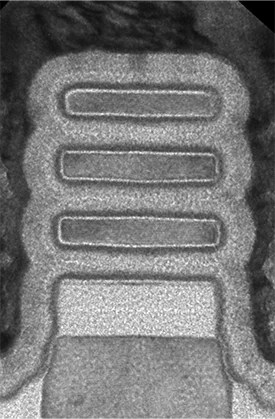
\includegraphics[width=24mm]{img/ibm2nm.png}
\end{marginfigure}
\marginnote{\bibentry{ibm2nm}}

\section{From Physical to Logical}

\begin{circuitikz}[scale=0.8, framed]
  \ctikzset{resistors/scale=0.4, font=\scriptsize};
  \draw
    (0,0) node[left] (top5v) {5V}
    to[short, o-, i=$ $]
    ++(1,0) coordinate(T)
    to[short]
    ++(0,-1) node[npn, anchor=C] (toptrans) {}
    (toptrans.E) to[short]
    ++(0,-1) node[npn, anchor=C] (bottrans) {}
    (bottrans.E)
    to[short, i=$ $]
    ++(0,-1) coordinate(X)
    to[R=$5k\Omega$, i=$ $]
    ++(0,-3) node[ground] {}
    
    (toptrans.B)
    to[R=$10k\Omega$, i<=$ $]
    ++(-3, 0) node[cuteopenswitchshape,anchor=1] (s1) {}
    (s1.in)
    to[short, -o, i<=$ $]
    ++(-1,0) node[left] {5V}
    
    (bottrans.B)
    to[R=$10k\Omega$, i<=$ $]
    ++(-3, 0) node[cuteopenswitchshape,anchor=1] (s2) {}
    (s2.in)
    to[short, -o, i<=$ $]
    ++(-1,0) node[left] {5V}
    
    (X)
    to[leD, *-, fill=red, i=$ $]
    ++(4,0) node {}
    to[short, i=$ $]
    ++(0,-3) node[ground] {}
    ;
\end{circuitikz}

\marginnote[-50mm]{\bibentry{circuitdigestandgate}}

\vspace{8mm}

\begin{circuitikz}[scale=0.8, framed]
  \ctikzset{font=\scriptsize};
  \draw (0,0) node[and port] {AND};
\end{circuitikz}


\end{document} 